\documentclass[14pt,letterpaper]{article}
\usepackage[utf8]{inputenc}
\usepackage[spanish]{babel}
\usepackage{times}
\usepackage[left=3cm,top=2.5cm,bottom=2.5cm,right=2.5cm]{geometry}
\usepackage{graphicx}
\author{Perez de Alba Santiago Eduardo.}

\begin{document}
\begin{center}

\LARGE \textbf{Universidad Politecnica de la Zona Metropoilitana de Guadalajara\\}


\includegraphics[scale=1]{Upzmg.png} 

\large \textbf{2\_ 5\_ arreglos\_ de\_ amplificadores\_ de\_ potencia.}

\end{center}

\vspace{1cm} 
\large \textbf{Nombre: \\Perez de Alba Santiago Eduardo.\\ Romero Jauregui Osvaldo\\
\vspace{0.5cm} Carrera: Ingeniería en Mecatronica.\\
\vspace{0.5cm} Materia: Sistemas Electrónicos de Interfaz.\\
\vspace{0.5cm} Curso: Septiembre-Noviembre del 2019.\\
\vspace{0.5cm} Docente: Moran Garabito Carlos Enrique.}\\
\vspace{0.5cm}
\small \textbf{07 de diciembre del 2019}


\newpage
\section{Introducción:}
Durante el desarrollo de estas simulación se irán explicando de que manera funcionan los diferentes Amplificadores Operacionales, como también se verán como desarrollarlos mediante un software para la predicción de resultados.

\section{Desarrollo:}
\subsection{Inversor:}
A este Amplificador se le llama asi debido a que la señal de salida es inversa a la de entrada, en polaridad, aunque esta puede ser mayor o menos dependiendo de la ganancia que tendrá el amplificador operacional en lazo cerrado.
\
Esto se da debido a nuestro voltaje de entrada y una resistencia en lazo (como antes mencionado), y una resistencia de a la entrada, por el cual circulara el voltaje.
\
Para calcular esta amplificación que tendrá nuestro circuito deberemos dividir nuestra resistencia de referencia que se encuentra en configuración de lazo, entre la resistencia de entrada al amplificador operacional, esto nos dará el resultado de amplificación que se espera.

$$G=\frac{-Rf}{Rin}$$
\
Donde:\\ G=Ganancia del circuito\\Rf= es la resistencia en lazo\\ Rin= es la resistencia de entrada
\
Dando como resultado -10

\subsection{No inversor:}
\
El amplificador no inversor permite amplificar una señal electrónica. por lo cual no altera la fase de entrada. A diferencia del Inversor es que en las entradas de voltaje sera direccionado al pin positivo mientras que la resistencia de lazo sera configurada en el pin negativo y tierra. Por lo tanto el calculo sera similar solamente con el cambio de nuestra resistencia de referencia de lado positivo.

$$G=\frac{Rf}{Rin}$$
\
Obteniendo como resultado el contrario del Inversor, entonces 10.
\
\subsection{Sumador:}
\
El amplificador sumador entrega en su salida de voltaje igual a la suma de los voltajes que tiene en sus entradas. Es decir, cada una de las entradas tiene una resistencia de entrada que al combinarse con la resistencia de realimentación forman un amplificador inversor de corriente continua de ganancia.
\
Este amplificador es similar al No inversor, con la diferencia que se agregan mas resistencias dependiendo del amplificador utilizado.
\
Uno de sus usos es en la suma de 2 o mas voltajes para esperar un solo voltaje de salida  demasiado grande debido a la suma de todos los voltaje en la entrada.\\ Para calcular el voltaje de salida es de la siguiente manera:
$$V_{out}=(\frac{V1}{R1}+\frac{V2}{R2}+\frac{V3}{R3}...+\frac{Vn}{Rn})$$

\
Donde:\\$V_{out}$= Voltaje de salida.
\\Vn=Es las fuente de voltaje.
\\Rn= Resistencia respecto a su fuente de voltaje.

\subsection{Restador:}
\
Este amplificador es una combinación entre el inversor y el no inversor con una ganancia de 1, para producir una salida igual a la diferencia entre las entradas, el cual resta las señal de una con las otras.
\
Para tener los voltajes de salida es de la siguiente manera:
$$V_{out}=V2(\frac{(R3+R3)(R4)}{(R4+R2)(R1)}-V1\frac{R3}{R1}$$

\
Donde:
\\$V_{out}$=Voltaje de salida
\\V2=Voltaje dos
\\V1=Voltaje uno
\\R1,R2,R3...Rn= Resistencia circuito.
\subsection{DAC:}
\
Un amplificador DAC es un convertidor de señales digitales a señales análogas, este esta conformado por un pulsador o switch o compuertas lógicas, con una resistencia para simular cada bit, dependiendo de los bits que se requieran son las lineas de resistencias y pulsadores, que al momento de pulsar se observe un incremento o un decremento en la señal de salida.
\
Para calcular la salidas de este se lleva por medio de valores lógicos (0 y 1) donde 1 serian 10V de entrada y 0 seria 0V:
$$R=\frac{1logico}{nBits}$$
\
Donde:
\\R= el valor de las resistencias en linea
\\1Logico= Voltaje de entrada
\\nBit= Los bits que queramos dentro de nuestro DAC.

\
\subsection{ADC:}
\
Este transforma señales analógicas en señales digitales. Funciona de manera que compara la función de una fuente con otra a través de sus valores lógicos, estos van variando dependiendo de nuestras resistencias conectadas en serie con switch o pulsador para reducir la resistencia de la misma, y así obtener una variación entre ambas fuentes integradas.
\
Para calcular nuestra salida y la conversión, es de la misma manera que el anterior, teniendo:
$$R=\frac{1logico}{nBits}$$
\
Donde:
\\R= el valor de las resistencias en linea
\\1Logico= Voltaje de entrada
\\nBit= Los bits que queramos dentro de nuestro DAC.
\newpage
\section{Resultados:}

\begin{figure}[h!]
\begin{center}
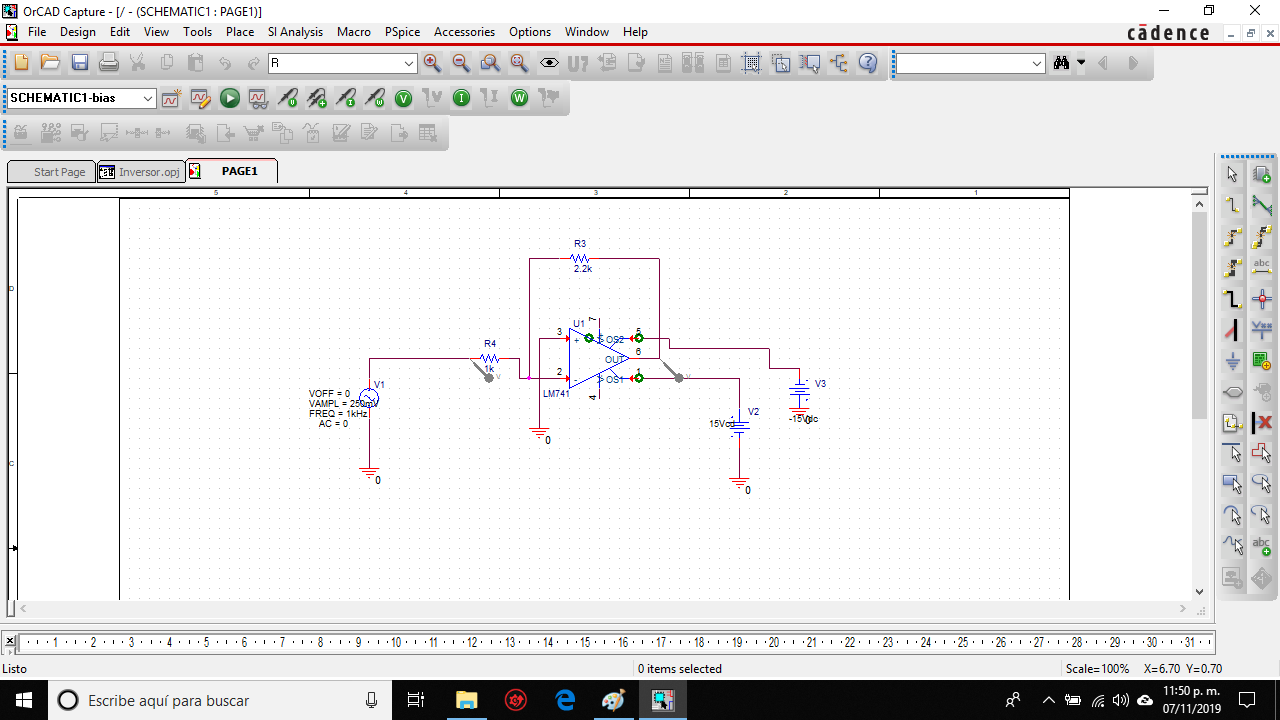
\includegraphics[scale=0.5]{Simulacion-PCB/inversor.png} 
\caption{Circuito Inversor.}
\end{center}
\end{figure}

\
\begin{figure}[h!]
\begin{center}
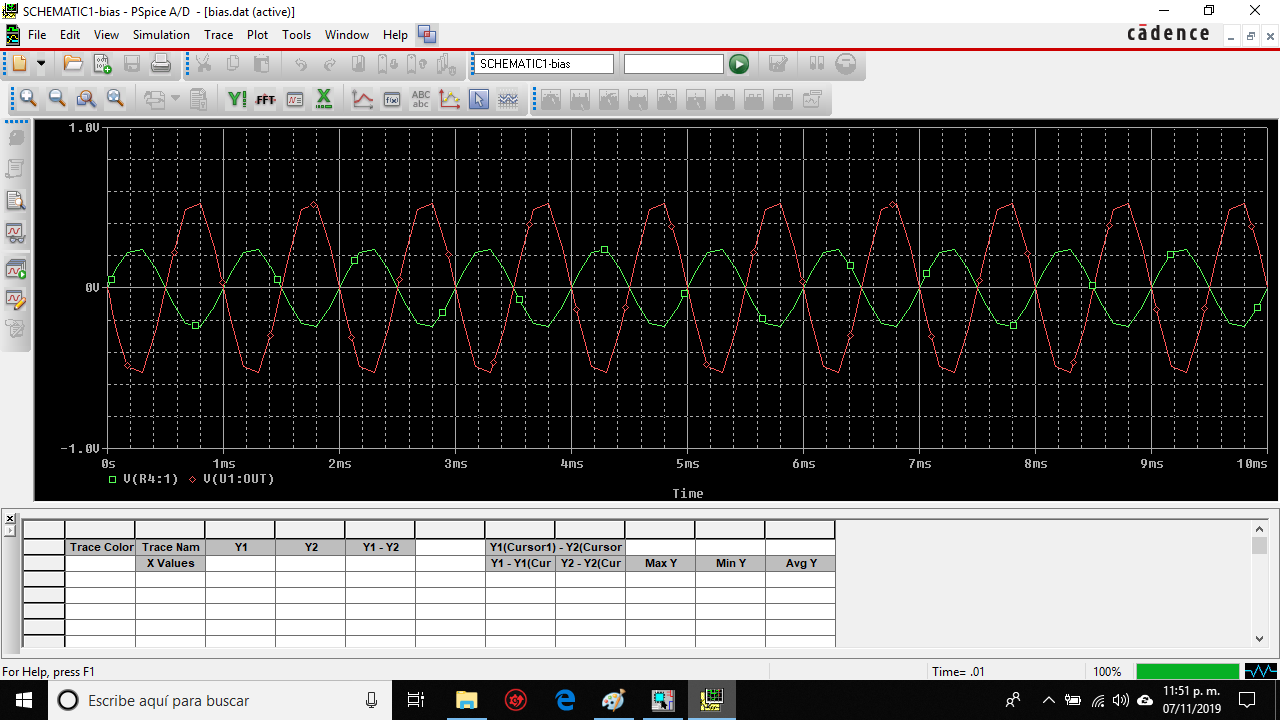
\includegraphics[scale=0.5]{Simulacion-PCB/siminversor.png} 
\caption{Simulación en PSpice Inversor.}
\end{center}
\end{figure}

\
\begin{figure}[h!]
\begin{center}
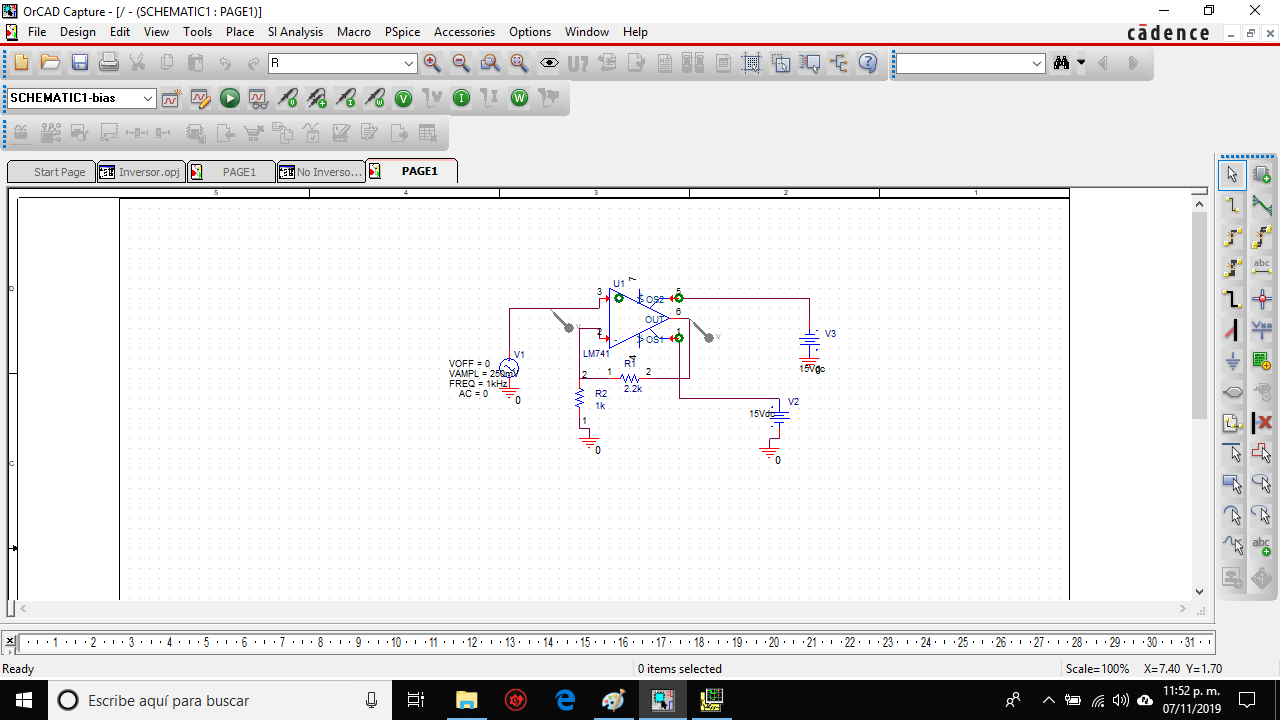
\includegraphics[scale=0.5]{Simulacion-PCB/noinversor.png} 
\caption{Circuito en OrCad de Amp Op. No Inversor.}
\end{center}
\end{figure}

\
\begin{figure}[h!]
\begin{center}
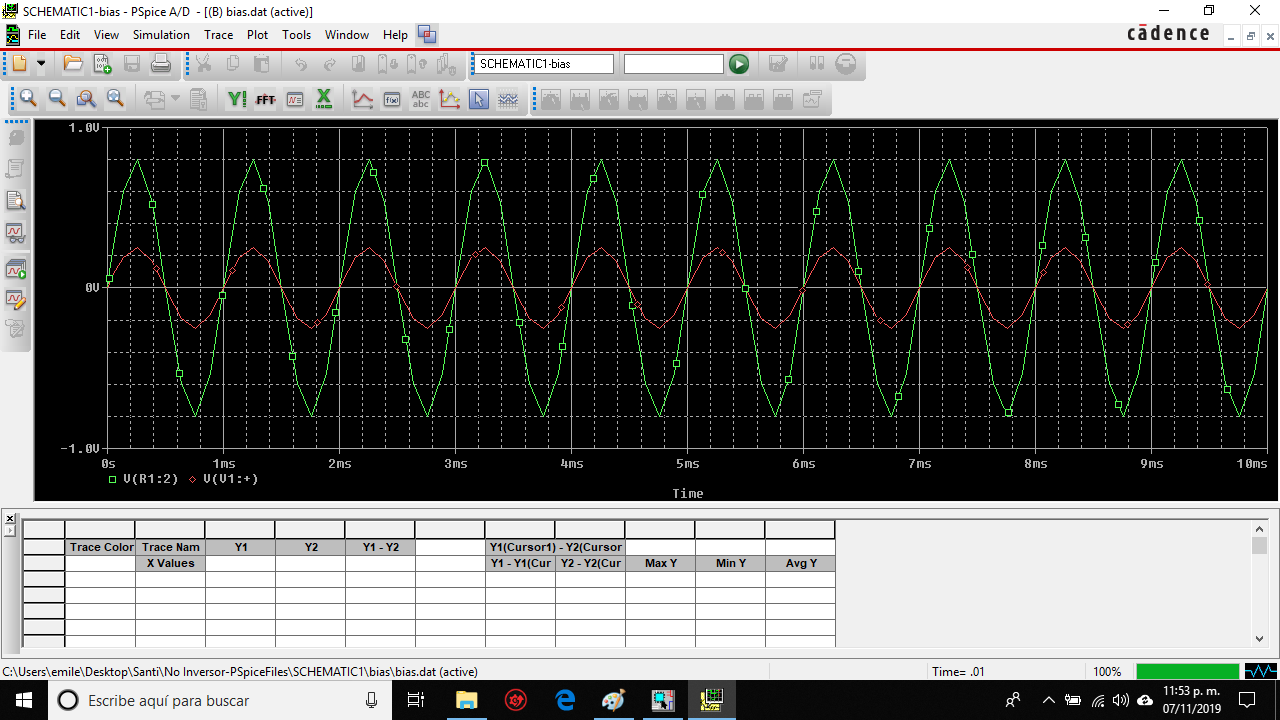
\includegraphics[scale=0.5]{Simulacion-PCB/simnoinversor.png} 
\caption{Simulación en PSpice Amp. Op. No inversor}
\end{center}
\end{figure}

\
\begin{figure}[h!]
\begin{center}
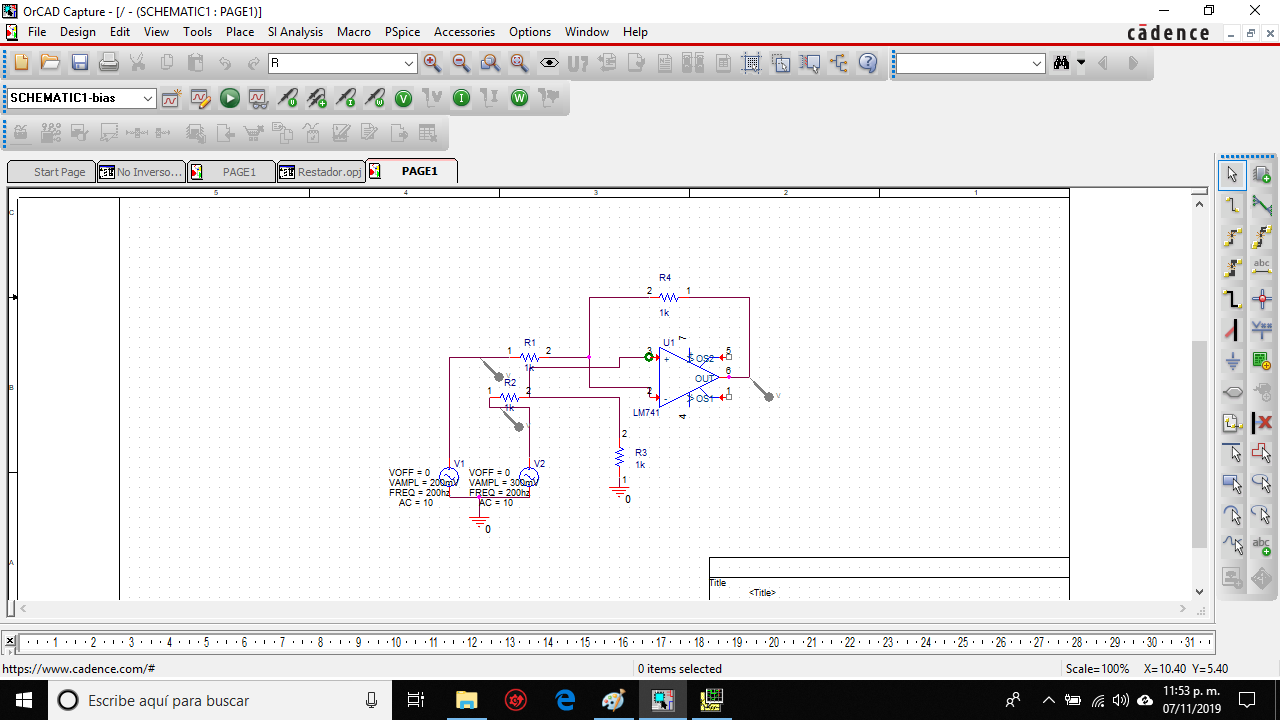
\includegraphics[scale=0.5]{Simulacion-PCB/restador.png} 
\caption{Simulación OrCad Amp. Op. Restador.}
\end{center}
\end{figure}

\
\begin{figure}[h!]
\begin{center}
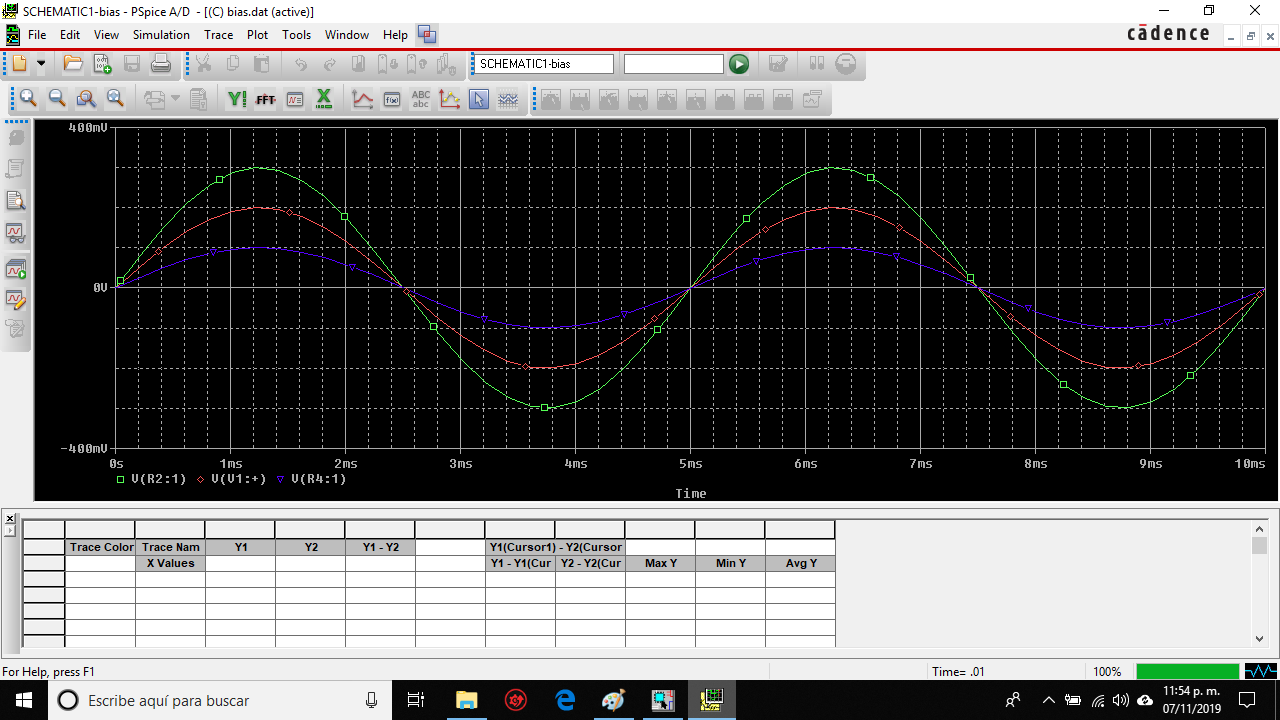
\includegraphics[scale=0.5]{Simulacion-PCB/simrestador.png} 
\caption{Simulación en PSpice Restador.}
\end{center}
\end{figure}

\
\begin{figure}[h!]
\begin{center}
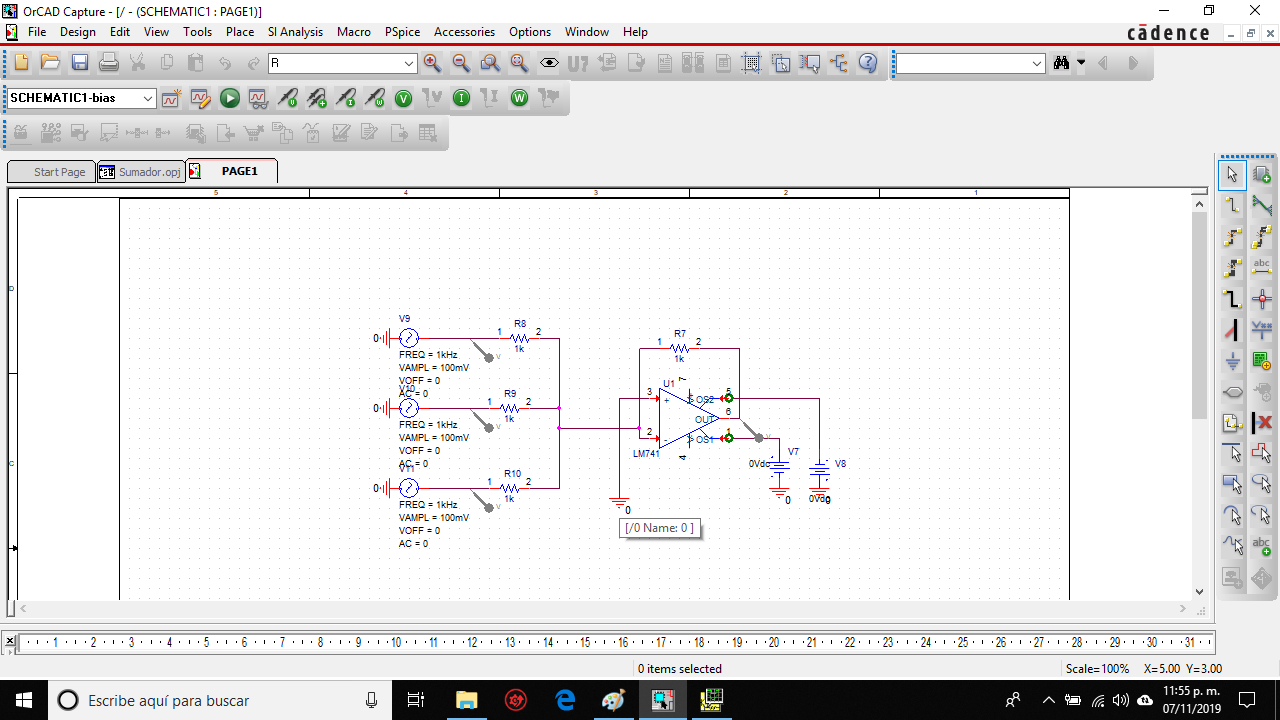
\includegraphics[scale=0.5]{Simulacion-PCB/sumador.png} 
\caption{Simulación OrCad del Amp. Op. Sumador.}
\end{center}
\end{figure}

\
\begin{figure}[h!]
\begin{center}
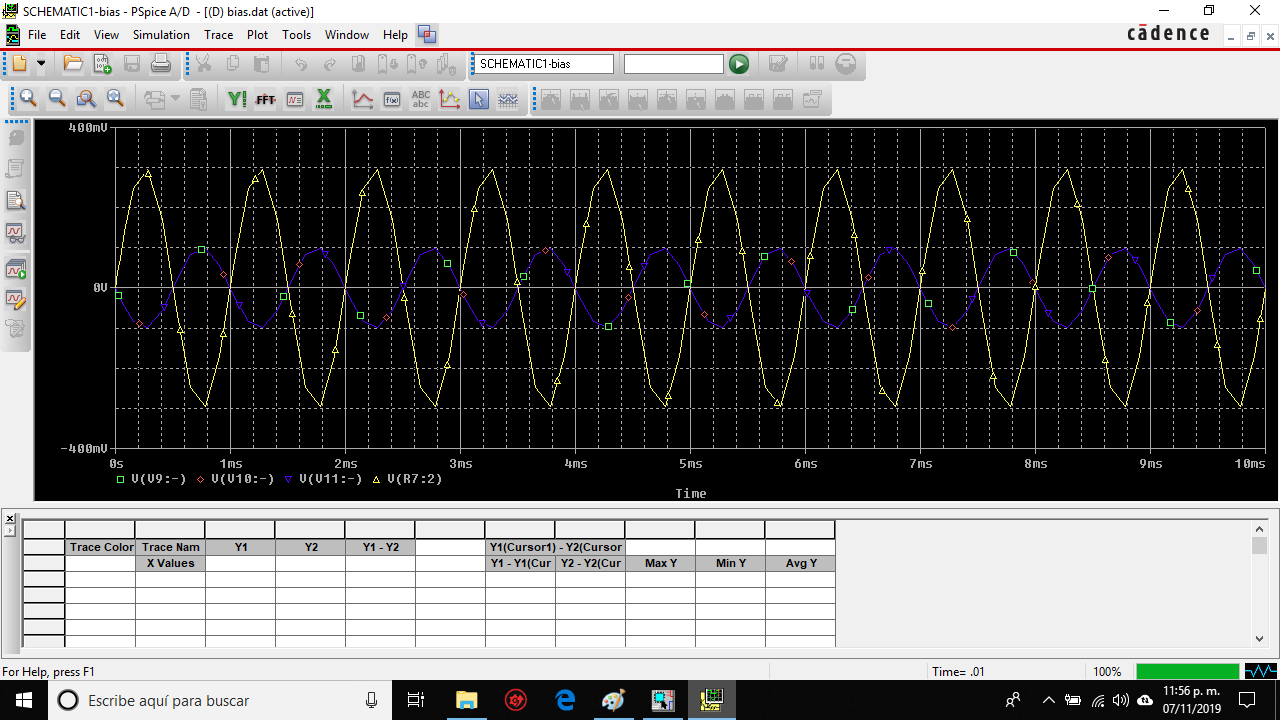
\includegraphics[scale=0.5]{Simulacion-PCB/simsumador.png}
\caption{Simulación PSpice de Amp. Op. Sumador} 
\end{center}
\end{figure}

\begin{figure}[h!]
\begin{center}
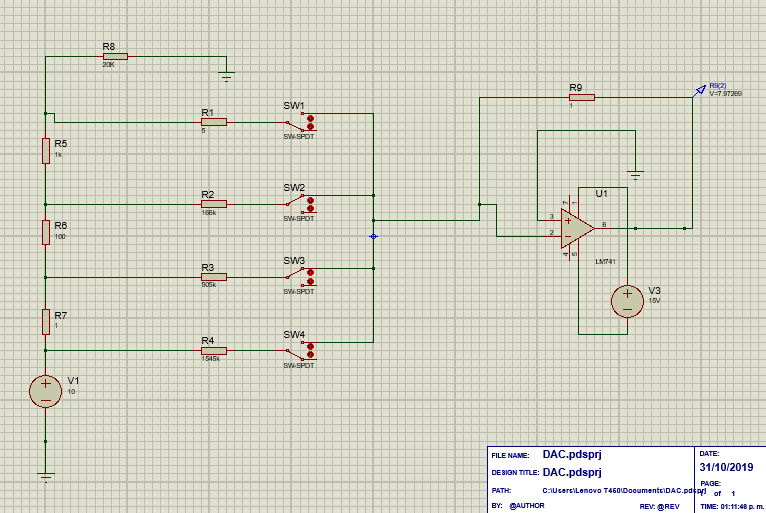
\includegraphics[scale=0.5]{Simulacion-PCB/dac.png} 
\caption{Circuito Proteus ADC}
\end{center}
\end{figure}
\
\begin{figure}[h!]
\begin{center}
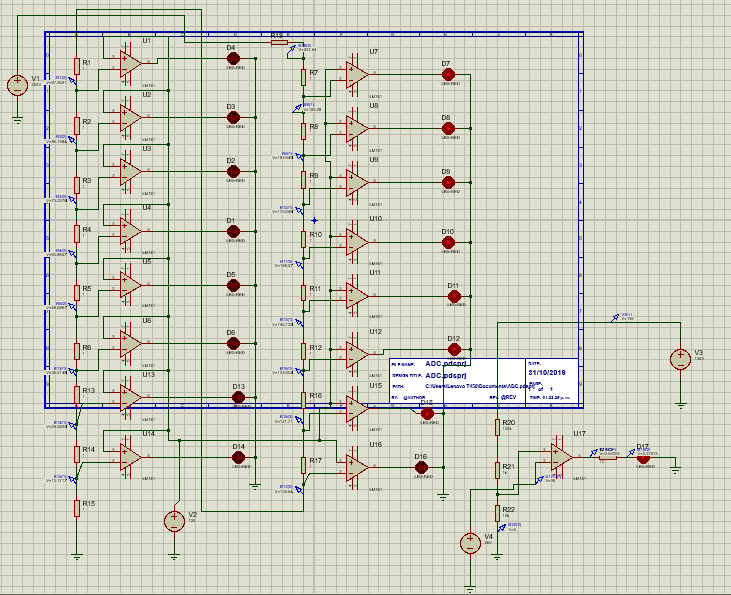
\includegraphics[scale=0.5]{Simulacion-PCB/simadc.png} 
\caption{Simulación Proteus ADC Voltaje variado.}
\end{center}
\end{figure}

\
\begin{figure}[h!]
\begin{center}
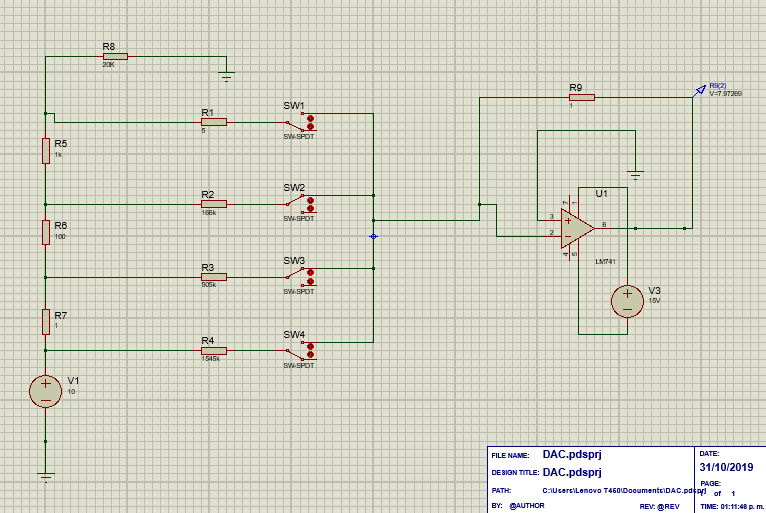
\includegraphics[scale=0.5]{Simulacion-PCB/dac.png}
\caption{Simulación Proteus DAC} 
\end{center}
\end{figure}

\
\begin{figure}[h!]
\begin{center}
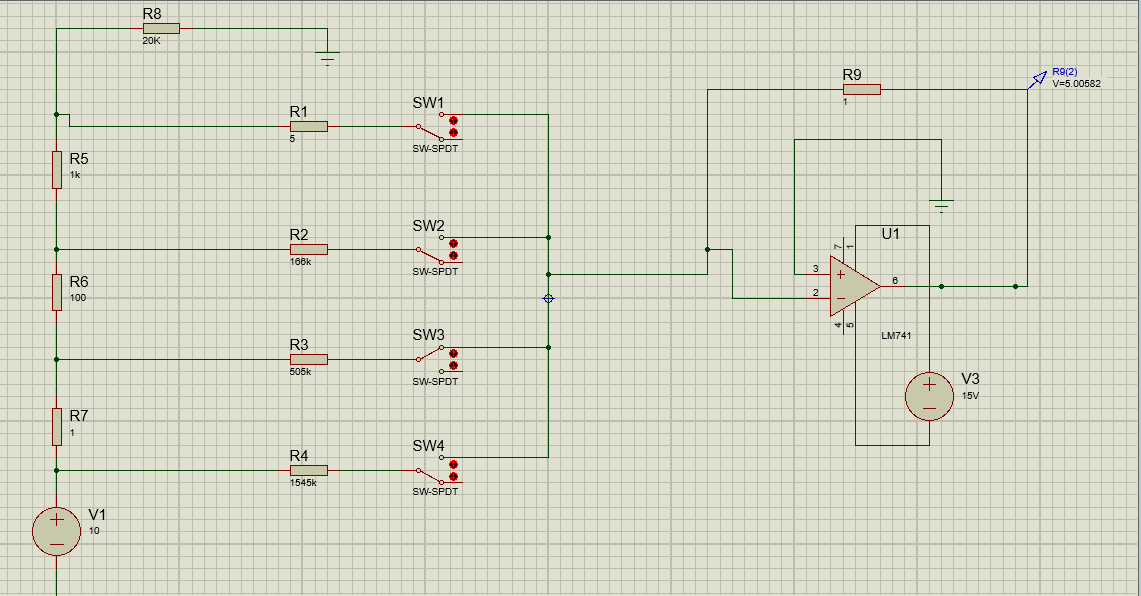
\includegraphics[scale=0.5]{Simulacion-PCB/simdac.png} 
\caption{Simulación Proteus de circuito DAC, Led encendidos y variación.}
\end{center}
\end{figure}

\section{Conclusion:}
\begin{itemize}
\item Durante la elaboración de las simulaciones pudimos observar de que manera funcionan los Amplificadores operacionales, en función de nuestras entradas de voltaje y resistencias que tengamos, pudimos observar la diferencia que provocaban los amplificadores en la salida a comparación de la entrada que dábamos.
\item Durante la elaboración de los Amplificadores operacionales se comprendieron diferentes significados y operaciones a las conocidas, pudimos observar de que manera varían las nuestras salidas al modificar nuestros valores de resistencia y al agregar algún obturador o interruptor para disminuir manualmente la resistencia y así aumentar o disminuir la ganancia de nuestro amplificador operacional.

\end{itemize}

\end{document}